\documentclass[../main.tex]{subfiles}

\begin{document}
%%%%%%%%%%%%%%%%%%%%%%%%%%%%%%%%%%%%%%%%%%%%%%%%%%%%
%                                                  %
% Differentialrechnung I -- Tangente und Ableitung %
%                                                  %
%%%%%%%%%%%%%%%%%%%%%%%%%%%%%%%%%%%%%%%%%%%%%%%%%%%%

\chapter{SW07 Differentialrechnung IV -- Kurvendiskussion, Optimierung}
\section{Parameterdarstellung von Kurven}
Neben der Form $y=f(x)$ kann man Kurven auch in der Parameterform beschreiben. 
Jedem Wert des Parameters t wird dabei ein Punkt $\vec{x}(t)$ in der Ebene (oder auch im Raum) zugeordnet. 
Man nennt dies auch Parameterdarstellung der Kurve.

\begin{minipage}{0.5\textwidth}
    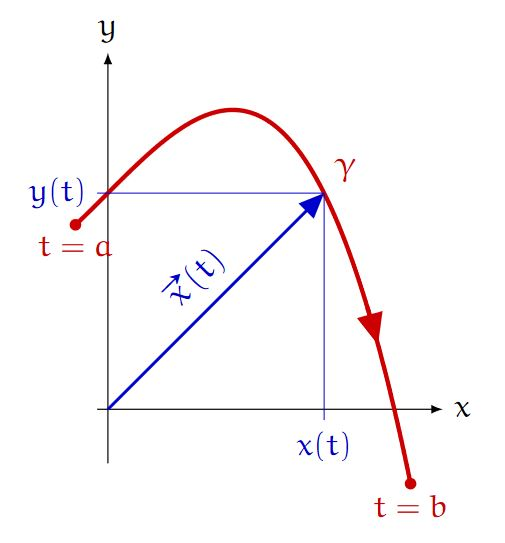
\includegraphics[width=50mm,scale=0.5]{parameterdarstellung}
\end{minipage} \hfill
\begin{minipage}{0.45\textwidth}
    Eine Kurve $\gamma$ ist eine Abb. der Form: \\ [7pt]
    $\gamma : [a,b] \to \mathbb{R}^2, t \mapsto \vec{x}(t)=
    \begin{bmatrix}
        x(t) \\
        y(t)
    \end{bmatrix}$ \\ [7pt]
    Für $t=a$ ist man am Kurvenanfang, für ein beliebiges $t \in [a,b]$ an der Stelle $\vec{x}(t)$ und für $t=b$ am Kurvenende. \\ [7pt]
    Für jeden Punkt $\vec{x}$ auf der Kurve gibt es genau ein $t \in [a,b]$ so, dass $\vec{x}(t)$ (und auch die Umkehrung gibt!)
\end{minipage}

\subsection{Beispiel}
Funktion: $f:[a,b] \to \mathbb{R}, x \mapsto y = f(x)$ \\
Parameter: $t=x$ \\
Parameterform: $\gamma : [a,b] \to \mathbb{R}^2, t \mapsto \vec{x}(t)=
\begin{bmatrix}
    t \\
    f(t)
\end{bmatrix}$ \\ [7pt]
Funktion: $y=x^2$ \\
$f: \mathbb{R} \to \mathbb{R}^+_0, x \mapsto x^2$ \\
Kurve: $c: \mathbb{R} \to \mathbb{R}x \mathbb{R}^+_0, t \mapsto
\begin{bmatrix}
    t \\
    t^2
\end{bmatrix}$

\subsection{Ableitung eines Vektors}
Einen Vektor $\vec{x}(t)$ leitet man nach dem Parameter $t$ ab, indem man jede Komponente des Vektors nach $t$ ableitet.

\subsection{Ableitung einer in Parameterform gegebenen Funktion}
\begin{minipage}{0.5\textwidth}
    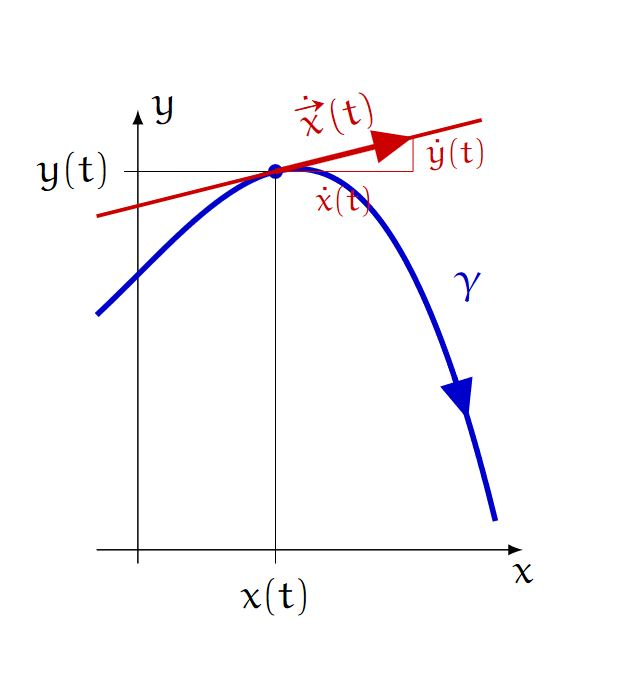
\includegraphics[width=50mm,scale=0.5]{parameterform_ableiten}
\end{minipage} \hfill
\begin{minipage}{0.45\textwidth}
    Parameterform der Kurve $\gamma$ \\ [7pt]
    $\vec{x}(t)=\begin{bmatrix}
        x(t) \\
        y(t)
    \end{bmatrix}, a \le t \le b$. \\ [7pt]
    Ist $\gamma$ gleich dem Graphen von $y=f(x)$ dann gilt für die Steigung der Tangente \\ [7pt]
    $y'=\frac{\dot{y}}{\dot{x}}$ \\ [7pt]
    wobei $\dot{y}$ die Ableitung von $y(t)$, bzw $\dot{x}$ von $x(t)$ nach $t$ ist.
\end{minipage}

Beachte: die Steigung der Tangente an $y'$ ist die selbe wie die Steigung des Vektors $\dot{\vec{x}}(t)$. 
Und diese lässt sich aus den beiden Komponenten $\dot{y}(t)$ und $\dot{x}(t)$ berechnen.

\subsection{Krümmungskreismittelpunkt}
\begin{minipage}{0.5\textwidth}
    \includegraphics[width=50mm,scale=0.5]{krümmungskreismittelpunkt}
\end{minipage} \hfill
\begin{minipage}{0.45\textwidth}
    Punkt auf der Kurve $\vec{x}(t)=[x,y(x)]^T$, 
    Tangente $\vec{t}=[1,y'(x)]^T$,
    Normale $\vec{n}(x)=[-y'(x),1]^T$.
    Mittelpunkt des Krümmungskreises (rot): \\ [7pt]
    $\vec{x}_M(x) = \vec{x}(x) + \frac{1}{K(x)}\frac{\vec{n}(x)}{|\vec{n}(x)|}$
\end{minipage}
Damit hat man für den Krümmungskreismittelpunkt: \\ [7pt]
\begin{math}
\vec{x}_M(x)=
\begin{bmatrix}
    x_M(x) \\
    y_M(x)
\end{bmatrix} = 
\begin{bmatrix}
    x-y'(x)\frac{1+(y'(x))^2}{y''(x)} \\
    y(x)+\frac{1+(y'(x))^2}{y''(x)}
\end{bmatrix}
\end{math}
wobei $K(x) = \frac{y''(x)}{(1+(y'(x))^2)^{\frac{3}{2}}}$

\section{Kurven in Polarkoordinaten}

Oft verwendet man anstelle der kartesischen Koordinaten $(x,y)$ Polarkoordinaten $(r, \phi)$.
Für die Koordinatentransformation gilt: \\ [7pt]
\begin{minipage}{0.5\textwidth}
    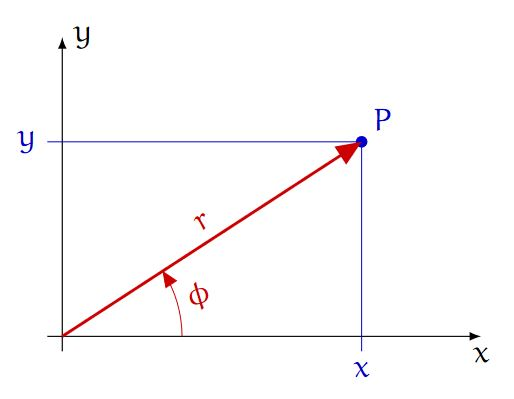
\includegraphics[width=50mm,scale=0.5]{polarkoordinaten}
\end{minipage} \hfill
\begin{minipage}{0.45\textwidth}
    \textbf{Polar- zu kartesischen Koordinaten:} \\ [7pt]
    $x = r \cos \phi$ \\ [7pt]
    $y = r \sin \phi$ \\ [7pt]
    \textbf{Kartesiche zu Polarkoordinaten:} \\ [7pt]
    $r=\sqrt{x^2 + y^2}$ \\ [7pt]
    $\tan \phi = \frac{y}{x}$
\end{minipage}
Beachte: Verwendet man $\phi = \arctan(\frac{y}{x})$ erhält man $\phi \in (\frac{-\pi}{2},\frac{\pi}{2})$.
Die Vorzeichen von $x$ und $y$ bestimmen, in welchem Quadranten der Punkt P liegt. 
Damit kann dann $\phi \in [0,2\pi]$ bestimmt werden. \\

\begin{minipage}{0.5\textwidth}
    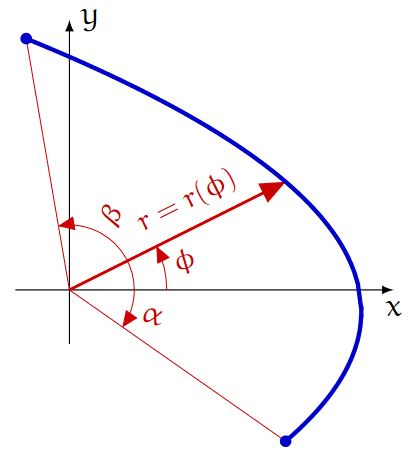
\includegraphics[width=50mm,scale=0.5]{polarkoordinaten2}
\end{minipage} \hfill
\begin{minipage}{0.45\textwidth}
    Eine in Polarkoordinaten gegebene Kurve $\gamma$ wird durch folgende Abbildung spezifiziert: \\
    $\gamma : [\alpha, \beta] \to \mathbb{R}, \phi \mapsto r = r(\phi)$ \\ [7pt]
    Jedem Winkel $\phi \in [\alpha, \beta]$ wird der Abstand der Kurve $r=r(\phi)$ vom Ursprung zugeordnet. \\ [7pt]
    Beachte: Alle Winkel werden von der positiven x-Achse im Gegenuhrzeigersinn gemessen. Hier ist damit $\alpha < 0$ und $\beta > 0$.
\end{minipage}

\subsection{Ableitung einer in Polarkoordinaten gegebene Funktion}
Die gewöhnliche Ableitung einer Funktion wird bestimmt, indem man die Polarkoordinaten in Parameterform transformiert \\ [7pt]
$x = x(\phi) = r(\phi)\cos \phi$ \\
$xy = y(\phi) = r(\phi)\sin \phi$ \\ [7pt]
Hier ist jetzt $\phi$ der Parameter. Formel $y'(x)=\frac{\dot{y}}{\dot{x}}$ \\ [7pt]
$y'(x)=\frac{dy}{dx}=\frac{\frac{dy}{d\phi}}{\frac{dx}{d\phi}}=\frac{\dot{r}(\phi)\sin \phi + r(\phi)\cos \phi}{\dot{r}(\phi)\cos \phi - r(\phi)\sin \phi}$

\section{Kurvendiskussion}
Generelles Vorgehen:
\begin{itemize}
    \item \textbf{Definitions- und Wertebereich, Definitionslücken, \\ Unstetigkeitsstellen}
    \item \textbf{Symmetrien:} ist f gerade $f(x)=f(-x)$, ungerade $f(x)=-f(-x)$ oder T-periodisch $f(x+T) = f(x)$.
    \item \textbf{Nullstellen} $f(x)=0$; \textbf{Schnittpunkte mit y-Achse} $f(0) = y$
    \item \textbf{Pole}: Nenner verschwindet; \textbf{senkrechte Asymptoten}: Polgeraden
    \item \textbf{Ableitungen} in der Regel bis zur 3. Ordnung
    \item \textbf{Relative Extremwerte} (Maxima, Minima): Notwendige Bedingung \\ $f'(x)=0$, $f''(x)>0$ = Minima, $f''(x)<0$ = Maxima.
    \item \textbf{Monotonieeigenschaften, Wendepunkte, Krümmung}
    \item \textbf{Asymptotisches Verhalten} für $x \to \pm \infty$
    \item \textbf{Krümmungskreismittelpunkt}
    \item \textbf{Graph G(f) der Funktion f skizzieren}
\end{itemize}

\subsection{Symmetrien Beispiele}
\begin{tabularx}{1.0\textwidth} { 
    >{\centering\arraybackslash}X 
    >{\centering\arraybackslash}X  }
    \hline
    Funktion & Bemerkung \\ [7pt]
    \hline
    $x^{2n}$ & Gerade: $x^2, x^4, x^6$... \\ [7pt]
    $x^{2n-1}$ & Ungerade: $x, x^3, x^5$...   \\ [7pt]
    $\cos 3x$ & Periodisch: $T=\frac{2\pi}{3}$ \\ [7pt]
    $e^{-x^2}$ & Gerade \\ [7pt]
    $\sin 2x$ & Ungerade, Periodisch $T=\pi$ \\ [7pt]
    $x^3\sin x$ & Gerade \\ [7pt]
    &
\end{tabularx}
In Quotient-funktion: Zähler gerade, Nenner ungerade = Funktion ungerade.

\subsection{Wende- und Sattelpunkte}
Notwendige und hinreichende Bedingung für einen Wendepunkt der Funktion $y=f(x)$ in $x_0$: \\
$f''(x_0) = 0$, und $f'''(x_0) \neq 0$. \\
Gilt zudem $f'(x_0) = 0$, dann hat man in $x_0$ einen Sattelpunkt.

\subsection{Beispiel}
\textbf{Funktion}: $y = \frac{-5x^2 + 5}{x^3}$ \\ [7pt]
\textbf{Definitions- und Wertebereich}: \\
 $D = \mathbb{R}$ \textbackslash $\{0\}, W = \mathbb{R}$ \\ [7pt]
\textbf{Symmetrie}: \\
Zähler gerade, Nenner ungerade = Funktion ungerade. \\ [7pt]
\textbf{Nullstellen}: \\
$y = \frac{-5x^2 + 5}{x^3} = 5 \frac{1-x^2}{x^3} = 5 \frac{(1+x)(1-x)}{x^3}$ \\ [7pt]
$x_{1,2} = -1,1$ \\ [7pt]
\textbf{Polstellen bei 0}: \\
$\lim\limits_{x \to 0^-} \frac{-5x^2+5}{x^3} = \frac{5}{0^-} = -\infty$ \\ [7pt]
$\lim\limits_{x \to 0^+} \frac{-5x^2+5}{x^3} = \frac{5}{0^+} = \infty$ \\ [7pt]
\textbf{Ableitungen}: \\
$y = \frac{-5x^2 + 5}{x^3}$ \\ [7pt]
$y' = 5\frac{x^2-3}{x^4}$ \\ [7pt]
$y'' = 5\frac{12 - 2x^2}{x^5}$ \\ [7pt]
$y''' = 30 \frac{x^2 - 10}{x^6}$ \\ [7pt]
\textbf{Extrema}: \\
$y' = 5\frac{x^2-3}{x^4} = 0; x^2-3=0; x_{1,2}=\pm\sqrt{3}$ \\ [7pt]
$y''(x_1)=y''(\sqrt{3}) = 5 \frac{12 - 2\sqrt{3}^2}{\sqrt{3}^5} > 0$ Minimum \\ [7pt]
$y''(x_2)=y''(-\sqrt{3}) = 5 \frac{12 - 2 \times -\sqrt{3}^2}{-\sqrt{3}^5} < 0$ Maximum \\ [7pt]
\textbf{Wendepunkte}: \\
$y'' = 5\frac{12 - 2x^2}{x^5} = 0; 12-2x^2=0; 6=x^2; x=\pm \sqrt{6}$ \\ [7pt]
$y'''(\pm \sqrt{6}) = 30 \frac{(\pm \sqrt{6})^2 - 10}{(\pm \sqrt{6})^6}
= 30 \frac{-4}{6^3} \neq 0$ \\ [7pt]
Wendepunkte bei $-\sqrt{6}$ und $\sqrt{6}$ \\ [7pt]
\textbf{Asymptotisches Verhalten}: \\
$\lim\limits_{x \to \infty} \frac{5-5x^2}{x^3} = \lim\limits_{x \to \infty} 5\frac{1-x^2}{x^3} 
= \lim\limits_{x \to \infty} 5(\frac{1}{x^3} - \frac{1}{x}) 
= 5 (\lim\limits_{x \to \infty} \frac{1}{x^3} - \lim\limits_{x \to \infty} \frac{1}{x}) = 0$

\section{Optimierungsproblem - Allgemeines Vorgehen}
Bei Extremalwertprobleme (oder Extremwert- oder Extremalaufgaben) sucht man einen 
Extremwert für ein bestimmtes Problem, zB maximales Volumen, minimale Distanz, etc.

\begin{itemize}
    \item Zuerst die Funktion bestimmen, welche das Problem beschreibt.
    \item Aus den Nullstellen der Ableitung ($f'(x)=0$) erhält man Kandidaten für Extrempunkte $x_0$
    (mit zugehörigen Extremwerten $f(x_0)$)
    \item Mit den höheren Ableitungen überprüft man, ob es sich um Minima, Maxima oder Sattelpunkte handelt: \\
    \textbf{Rel. Max in $x_0$}: $f^{(n)}(x_0)<0$, n gerade und $f^{(k)}(x_0)=0$, für $1 \leq k < n$ \\
    \textbf{Rel. Min in $x_0$}: $f^{(n)}(x_0)>0$, n gerade und $f^{(k)}(x_0)=0$, für $1 \leq k < n$
    \textbf{Sattelpunkt $x_0$}: $f^{(n)}(x_0) \neq 0$, n ungerade \\
    und $f^{(k)}(x_0)=0$, für $2 \leq k < n$ 
    \item Die Funktionswerte der gefundenen Maxima (Minima) und die Werte der Funktion an den Rändern werden 
    jetzt verglichen. Das grösste (kleinste) ist der gesuchte Extremwert.
\end{itemize}

\subsection{Brechungsgesetz}
???


\section{Regel von de l'Hôpital}
\subsection{Theorem - Regel von de l'Hôpital für unbestimmte Ausdrücke der Form 0/0}
Wir nehmen an $f$ und $g$ seien in einer Umgebung von $x=a$ differenzierbar und $\lim\limits_{x \to a}f(x)=0$
und $\lim\limits_{x \to a}g(x)=0$. Dann gilt $\lim\limits_{x \to a}\frac{f(x)}{g(x)} = \lim\limits_{x \to a}\frac{f'(x)}{g'(x)}$
falls die rechte Seite existiert oder $\pm \infty$ ist. \\
Weiter gilt die Regel auch für die Grenzübergänge $x \to a^-,x \to a^+, x \to +\infty,x \to -\infty$.

\subsection{Vorgehen}
\begin{itemize}
    \item Überprüfe, ob $\lim\limits_{x \to a}\frac{f(x)}{g(x)}$ ein unbestimmter Ausdruck der Form 0/0 ist.
    \item Wenn ja, leite f und g separat ab.
    \item bestimme den Grenzwert $\lim\limits_{x \to a}\frac{f'(x)}{g'(x)}$. Wenn dieser endlich ist oder $\pm \infty$, dann ist dies der gesuchte Grenzwert.
\end{itemize}

\subsection{Vorgehen für weitere unbestimmte Ausdrücke}
\begin{itemize}
    \item Satz gilt entsprechend auch für unbestimmte Ausdrücke der Form $\frac{\infty}{\infty}$ 
    \item Unbestimmte Ausdrücke der Form $0 \times \infty$ bringt man mittels der Identität \\
    $f(x)g(x)=\frac{f(x)}{\frac{1}{g(x)}}$ auf einen unbestimmten Ausdruck der Form 0/0.
    \item Unbestimmte Ausdrücke der Form $\infty - \infty$ lassen sich of durch geeignete algebraische 
    Umformungen auf unbestimmte Ausdrücke der Form 0/0 zurückführen.
    \item Unbestimmte Ausdrücke der Form $0^0, \infty^0, 1^\infty$ schreiben wir in der Form $y=f(x)^{g(x)}$,
    logarithmieren beide Seiten und erhalten dann mit $ln y=g(x) \times ln(f(x))$ einen der oben besprochenen Ausdrücke.
\end{itemize}


\end{document}